
\documentclass{../concepts/titul_protokol_p/prepareprotokol} %všechny balíčky pro protokol + titulní strana
\renewcommand{\today}{\number\day.\,\number\month.\,\number\year}
\usepackage{graphicx}
\usepackage{newfloat}
\usepackage{caption}
\usepackage{booktabs}
\usepackage{amssymb}
\usepackage{amsmath}
\usepackage{newfloat}
\usepackage{caption}
\usepackage{siunitx}
\usepackage{textcomp}
\usepackage{gensymb}
\sisetup{inter-unit-product =$\cdot$}
\sisetup{separate-uncertainty=true}

\praktikum{III} %číslo praktika (I, II nebo III)
\autor{David Němec} %jméno autora
\datum{24.\,2.\,2026} %datum měření
\cislo{16} %číslo úlohy
\nazev{Měření indexu lomu Fraunhoferovou metodou} %název úlohy

\DeclareFloatingEnvironment[fileext=los, placement={htbp}, name=Obrázek]{schema}

\newcommand{\nobars}{
Chybové úsečky nebyly pro~svou malou velikost pro~přehlednost vykresleny.}

\newcommand{\relative}[1]{
\frac{\sigma_{#1}}{#1}
}
\newcommand{\squared}[1]{
\left( #1 \right)^2
}
\newcommand{\relsqr}[1]{
\squared{\relative{#1}}
%\left( \frac{\sigma_{#1}}{#1} \right)^2
}

\begin{document}
\renewcommand{\figurename}{Graf}
\renewcommand{\refname}{Literatura}

% add another graphics path to find ZPF.pdf for title page
% now searches for images in ./ and ../concepts/titul_protokol_p/
\graphicspath{{../concepts/titul_protokol_p/}}
\maketitle

% ========================== PRACOVNÍ ÚKOL ============================
\section{Pracovní úkol}
\begin{enumerate}
    \item Seřiďte goniometr.
    \item Změřte lámavý úhel skleněného hranolu a proměřte indexy lomu čar spektra rtuťové výbojky.
    \item Naměřené hodnoty zpracujte graficky do disperzní křivky. Graf vytvořte v praktiku, je povinnou součástí zápisu z měření.
    \item Vypočtěte střední disperzi, relativní disperzi a Abbeovo číslo pro měřený materiál, proveďte srovnání s tabelovanými hodnotami optických skel.
    \item Odvoďte výraz pro chybu nepřímého měření indexu lomu. Spočtěte její velikost a diskutujte, kolik desetinných míst indexu lomu tato metoda zaručuje.
\end{enumerate}

% ============================= TEORIE ================================
\section{Teorie}
\subsection{Určení lámavého úhlu hranolu}

Při fixní pozici hranolu lze lámavý úhel $\varphi$ u jedné vybrané hrany určit změřením 
úhlů $\alpha_1$ a $\alpha_2$, které odpovídají pozicím dalekohledu, kdy je optická osa 
dalekohledu přesně kolmá na~jednu ze~stěn hranolu, které jsou přilehlé k vybrané hraně.
Lámavý úhel se pak vypočítá podle vzorce \cite{pokyny}
\begin{equation}\label{eq:lamavyuhel}
    \varphi = |180\degree - |\alpha_1 - \alpha_2||\,.
\end{equation}

\subsection{Index lomu hranolu}

\begin{schema}
    \centering
    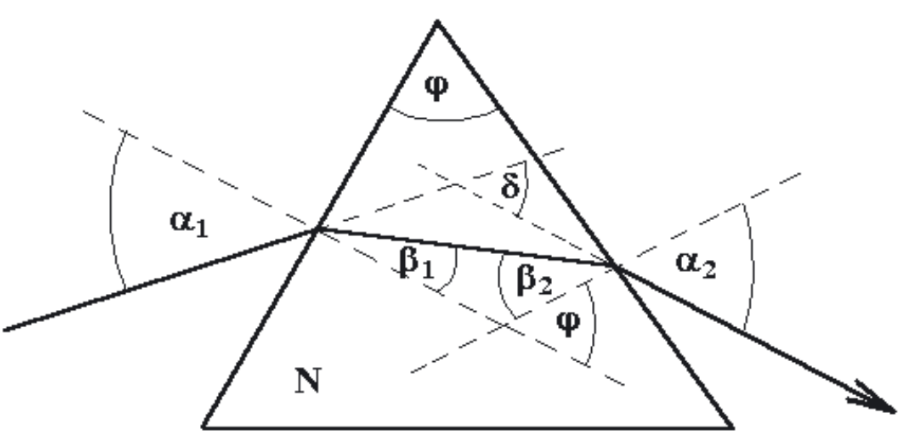
\includegraphics[width=0.5\linewidth]{hranol.png}
    \caption{Schéma průchodu paprsku skleněným hranolem. \cite{studijni}}
    \label{sch:hranol}
\end{schema}

Schéma průchodu paprsku hranolem o indexu lomu $N$ umístěného ve vzduchu o indexu 
lomu $N_0 = 1$ je znázorněno na~obrázku \ref{sch:hranol}. Při nastavení
sestavy do takové polohy, kdy je úhel odklonu $\delta$ dané vlnové délky minimální,
lze z geometrie a zákona lomu odvodit vztah pro index lomu hranolu $N$ \cite{pokyny}:
\begin{equation}\label{eq:indexlomu}
    N = \frac{\sin \left( \frac{\delta_{min} + \varphi}{2} \right)}{\sin \left(
        \frac{\varphi}{2} \right)} \, ,
\end{equation}
kde $\delta_{min}$ je minimální úhel odklonu a $\varphi$ je lámavý úhel hranolu.
Úhel odklonu $\delta_{min}$ se v tomto případě určí jako polovina vzdálenosti mezi
dvěma pozicemi dalekohledu ($\beta_1$ a $\beta_2$), které odpovídají dvěma 
orientacím hranolu vůči kolimátoru (viz obr. \ref{sch:deltamin}),
tedy podle vztahu \cite{pokyny}:
\begin{equation}\label{eq:deltamin}
    \delta_{min} = \frac{| \beta_1 - \beta_2 |}{2}\,.
\end{equation}

\begin{schema}[htbp]
    \centering
    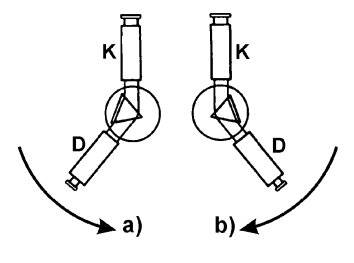
\includegraphics[width=0.5\linewidth]{minimalni_odchylka.png}
    \caption{Postup při určování minimálního úhlu odklonu (K je kolimátor,
    D dalekohled). \cite{pokyny}}
    \label{sch:deltamin}
\end{schema}

\subsection{Disperze a vlastnosti hranolu}

Jelikož index lomu hranolu závisí na vlnové délce světla, lze studovat disperzní
vlastnosti hranolu prostřednictvím tzv. disperzní křivky, která právě tuto
závislost $N = N(\lambda)$ znázorňuje. Přibližně ji lze popsat funkcí \cite{studijni}
\begin{equation}\label{eq:disperze}
    N(\lambda) = N_0 + \frac{a}{\lambda + \lambda_0}\, ,
\end{equation}
kde $N_0$, $a$ a $\lambda_0$ jsou parametry dané vlastnostmi hranolu.

Základní vlastnosti hranolu lze standardně charakterizovat pomocí
střední disperze, relativní disperze a Abbeova čísla.
Střední disperze $\Delta$ je definována jako \cite{studijni}
\begin{equation}\label{eq:Delta}
    \Delta = N_F - N_C\, ,
\end{equation}
kde $N_F$ a $N_C$ jsou indexy lomu spektrálních čar F a C, odpovídajících vlnovým délkám
$\lambda_F = 486.1\,\mathrm{nm}$ a $\lambda_C = 656.3\,\mathrm{nm}$ \cite{studijni}.

Relativní disperze $\delta$ se vypočítá jako \cite{studijni}
\begin{equation}\label{eq:delta}
    \delta = \frac{\Delta}{N_D - 1} = \frac{N_F - N_C}{N_D - 1}\, ,
\end{equation}
kde $N_D$ je index lomu spektrální čáry D o vlnové délce $\lambda_D = 589.3\,\mathrm{nm}$ 
\cite{studijni}.

Abbeovo číslo $\gamma$ se pak definuje pomocí relativní disperze jako \cite{studijni}
\begin{equation}\label{eq:gamma}
    \gamma = \frac{1}{\delta} = \frac{N_D - 1}{N_F - N_C}\,.
\end{equation}

\subsection{Metoda měření}

Schéma měřicí sestavy je znázorněno na~obrázku \ref{sch:goniometr}. Kolimátor
usměrní světlo rtuťové výbojky procházející štěrbinou do~rovnoběžného svazku, 
který následně dopadá na~skleněný hranol. Láme se na dvou stěnách hranolu,
které jsou odchýleny o lámavý úhel $\varphi$. Lomený paprsek se pak pozoruje otočným 
dalekohledem.

\begin{schema}[htbp]
    \centering
    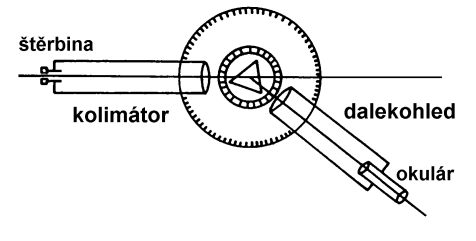
\includegraphics[width=0.5\linewidth]{goniometr.png}
    \caption{Schéma goniometru. \cite{pokyny}}
    \label{sch:goniometr}
\end{schema}

Před měřením bylo potřeba především pomocí šroubů seřídit podložku s hranolem tak, 
aby obě lámavé plochy hranolu byly kolmé na~optickou osu kolimátoru i~dalekohledu. 
To se dalo ověřit pozorováním obrazu nitkového kříže (odraženého od stěny hranolu), 
který se musel nacházet na nulové pozici svislé stupnice v dalekohledu, a~to 
i~při~otočení stolku s hranolem o 180\degree.

Lámavý úhel hranolu $\varphi$ se určil změřením dvou pozic dalekohledu, při kterých
je jedna či~druhá lámavá plocha hranolu kolmá na~optickou osu dalekohledu. Podložka
s hranole je v tomto případě nehybná.

Následně byl hranol natočen tak, aby se byly paprsky odchylovány o~minimální úhel.
Na okolí ideální pozice se~(při~synchronním otáčení dalehohledu společně s~hranolem) 
spektrum v~dalekohledu pohybovalo jedním směrem, zastavilo se a následně pohybovalo
opačným směrem. Právě v~krajní pozici je úhel odklonu minimální. Poté byla určitá 
spektrální čára jemným otočením dalekohledu nastavena do počátku stupnice v dalekohledu
a byla zaznamenána pozice dalekohledu $\beta_1$. Po proměření celého
spektra byl hranol otočen tak, aby paprsky vstupovaly do~lámavé plochy, ze~které 
předtím vystupovaly (obr. \ref{sch:deltamin}) a~postup se~opakoval. Minimální
úhel odklonu $\delta_{min}$ se~pak~určil jako polovina vzdálenosti mezi pozicemi
dalekohledu $\beta_1$ a $\beta_2$.


\subsection{Měřicí přístroje a jejich nejistoty}
%\begin{enumerate}
%    \item Goniometr SGO 1.1:
    
    \textbf{Goniometr SGO 1.1:} Goniometrem byly měřeny úhly natočení dalekohledu ($\alpha$ a $\beta$), ze kterých 
    byly následně vypočítány lámavý úhel hranolu a minimální úhel odklonu hranolu pro 
    paprsky jednotlivých spektrálních čar. Stupnice umožnovala odečítat úhly s přesností 
    na~2 úhlové vteřiny. K tomu by však bylo nutné přesně nastavit referenční čárku 
    mezi dva dílky stupnice, což nebylo úplně jednoduché. Z toho důvodu odhaduji nejistotu 
    měření úhlu jako 5 úhlových vteřin ($\sigma_{\alpha} = \sigma_{\beta} = 5\unit{\arcsecond}$).

%\end{enumerate}


% ======================== VÝSLEDKY MĚŘENÍ ===========================
\section{Výsledky měření}

\subsection{Lámavý úhel}
Nejprve byl určen lámavý úhel hranolu změřením dvou pozic dalekohledu,
při kterých byla jedna či~druhá lámavá plocha hranolu přesně kolmá
na~optickou osu dalekohledu. Byly změřeny úhly 
$\alpha_1 = 100.6597(14) \,\degree$ a $\alpha_2 = 220.6539(14) \,\degree$.
Podle vztahu (\ref{eq:lamavyuhel}) byl vypočten lámavý úhel hranolu
$\varphi = 60.006(2) \,\degree$, přičemž nejistota byla určena podle 
\cite{englich} jako
\begin{equation}\label{sigmaphi}
    \sigma_{\varphi} = \sqrt{2} \sigma_{\alpha} \, ,
\end{equation}
kde $\sigma_{\alpha} = 5\unit{\arcsecond}$ je nejistota měření úhlu $\alpha$.

\subsection{Index lomu}
Následně probíhalo přímo měření úhlu odklonu paprsků jednotlivých
spetkrálních čar rtuti. Pro obě orientace lámavých ploch hranolu,
které přiléhají k lámavému úhlu (obr. \ref{sch:deltamin}) byly
změřeny pozice dalekohledu $\beta_1$ a $\beta_2$, pro~které byla
určitá spektrální čára přesně v počátku horizontální stupnice 
dalekohledu. Minimální úhel odklonu $\delta_{min}$ pak byl určen
podle vztahu (\ref{eq:deltamin}) a jeho nejistota byla vypočtena
podle \cite{englich} jako
\begin{equation}\label{sigmadeltamin}
    \sigma_{\delta_{min}} = \frac{\sqrt{2}}{2} \sigma_{\beta} \, .
\end{equation}

Z úhlu odklonu a lámavého úhlu hranolu byl podle vzorce 
(\ref{eq:indexlomu}) vypočítán index lomu pro jednotlivé spektrální
čáry. Nejistota indexu lomu byla určena pomocí vzorce pro chybu nepřímého
měření, odvozeného z~obecného vzorce v~\cite{englich}:
\begin{equation}\label{eq:sigmaN}
    \sigma_N = \frac{1}{2 \sin \left(\frac{\varphi}{2}\right)} \sqrt{ 
    \cos^2 \left(\frac{\delta_{min} + \varphi}{2}\right)
    \sigma_{\delta_{min}}^2 + \frac{\sin^2 
    \left(\frac{\delta_{min}}{2}\right)}{\sin^2 
    \left(\frac{\varphi}{2}\right)}
    \sigma_\varphi^2 } \, .
\end{equation}

Změřené pozice dalekohledu, minimální úhly odklonu, vypočtené indexy
lomu a~tabelované vlnové délky (podle \cite{tabulka}) pro~jednotlivé
spektrální čáry rtuti shrnuje tabulka \ref{tab:rtut}.

\begin{table}[!htbp]
\centering
\caption{Naměřené úhly odklonu spektrálních čar rtuti, 
minimální úhel, odpovídající index lomu a tabelovaná vlnová délka
podle \cite{tabulka}}
\begin{tabular}{cccccc}
 \toprule
 barva & $\beta_1\, (\mathrm{\degree})$ & $\beta_2\, (\mathrm{\degree})$ & $\delta_{min}\, (\mathrm{\degree})$ & $\mathrm{N}$ & $\lambda\, (\mathrm{nm})$ \\
 \midrule
 červená & $200.0611(14)$ & $123.3767(14)$ & $38.342(1)$ & $1.51326(5)$ & $690.7$ \\
 červená & $200.1106(14)$ & $123.3256(14)$ & $38.393(1)$ & $1.51384(5)$ & $671.6$ \\
 červená & $200.2472(14)$ & $123.1894(14)$ & $38.529(1)$ & $1.51539(5)$ & $623.4$ \\
 červená & $200.2806(14)$ & $123.1583(14)$ & $38.561(1)$ & $1.51576(5)$ & $612.3$ \\
 červená & $200.2978(14)$ & $123.1372(14)$ & $38.580(1)$ & $1.51598(5)$ & $607.3$ \\
 žlutá & $200.3972(14)$ & $123.0383(14)$ & $38.679(1)$ & $1.51711(5)$ & $579.1$ \\
 žlutá & $200.4083(14)$ & $123.0303(14)$ & $38.689(1)$ & $1.51721(5)$ & $577.0$ \\
 zelená & $200.5367(14)$ & $122.9017(14)$ & $38.818(1)$ & $1.51867(5)$ & $546.1$ \\
 modrozelená & $200.8239(14)$ & $122.6117(14)$ & $39.106(1)$ & $1.52195(5)$ & $491.6$ \\
 modrá & $201.2411(14)$ & $122.1975(14)$ & $39.522(1)$ & $1.52664(5)$ & $435.8$ \\
 modrá & $201.2494(14)$ & $122.1811(14)$ & $39.534(1)$ & $1.52678(5)$ & $434.8$ \\
 modrá & $201.2550(14)$ & $122.1781(14)$ & $39.538(1)$ & $1.52683(5)$ & $433.9$ \\
 fialová & $201.5183(14)$ & $121.9172(14)$ & $39.801(1)$ & $1.52978(5)$ & $407.8$ \\
 fialová & $201.5614(14)$ & $121.8742(14)$ & $39.844(1)$ & $1.53026(5)$ & $404.7$ \\
 \bottomrule
\end{tabular}
\label{tab:rtut}
\end{table}

\subsection{Disperzní křivka a vlastnosti hranolu}

Závislost indexu lomu na~tabelované vlnové délce je pak vynesena
do~disperzní křivky na~obrázku \ref{fig:dispersion}. Datovými
body byla proložena křivka odpovídající funkci (\ref{eq:disperze}).
Koeficienty $N_0$, $a$ a $\lambda_0$ byly získány metodou
nejmenších čtverců pro~nelineární závislosti pomocí funkce
\texttt{curve\_fit} z~knihovny \texttt{scipy.optimize} jazyka Python.
Vycházejí jako $N_0 = 1.4990(3)$, $a = 7.5(2)\,\unit{nm^{-1}}$ a 
$\lambda_0 = -164(5)\,\unit{nm}$. Koeficient $a$ je kladný,
hranol tedy vykazuje normální disperzi.

Ke zjištění charakteristických vlastností hranolu byly vypočteny
indexy lomu významných spektrálních čar C, d, D a F, a~to dosazením 
jejich vlnových délek a koeficientů
$N_0$, $a$ a $\lambda_0$ do~vzorce (\ref{eq:disperze}).
Vlnové délky těchto spektrálních čar (převzatých z~\cite{studijni})
a odpovídající indexy lomu jsou shrnuty v tabulce \ref{tab:cdf}.
Nejistota indexu lomu pro~každou z~těchto spektrálních čar byla 
určena podle \cite{englich} jako (nejistotu tabelované vlnové délky neuvažuji)
\begin{equation}\label{eq:sigmaN2}
    \sigma_{N_i} = \sqrt{ \sigma_{N_0}^2 + \frac{\sigma_a^2}
    {\squared{\lambda_i + \lambda_0}} + \frac{ a^2 \sigma_{\lambda_0}^2}
    {\left( \lambda_i + \lambda_0 \right)^4}} , \quad
    i \in \{\mathrm{C}, \mathrm{d}, \mathrm{D}, \mathrm{F}\} \, .
\end{equation}

Index lomu spektrální čáry d Helia není důležitý pro~výpočet
parametrů střední disperze, relativní disperze a~Abbeova čísla,
využil jsem ho však při~určování typu skla použitého hranolu (viz
Diskuzi).

\begin{figure}
    \centering
    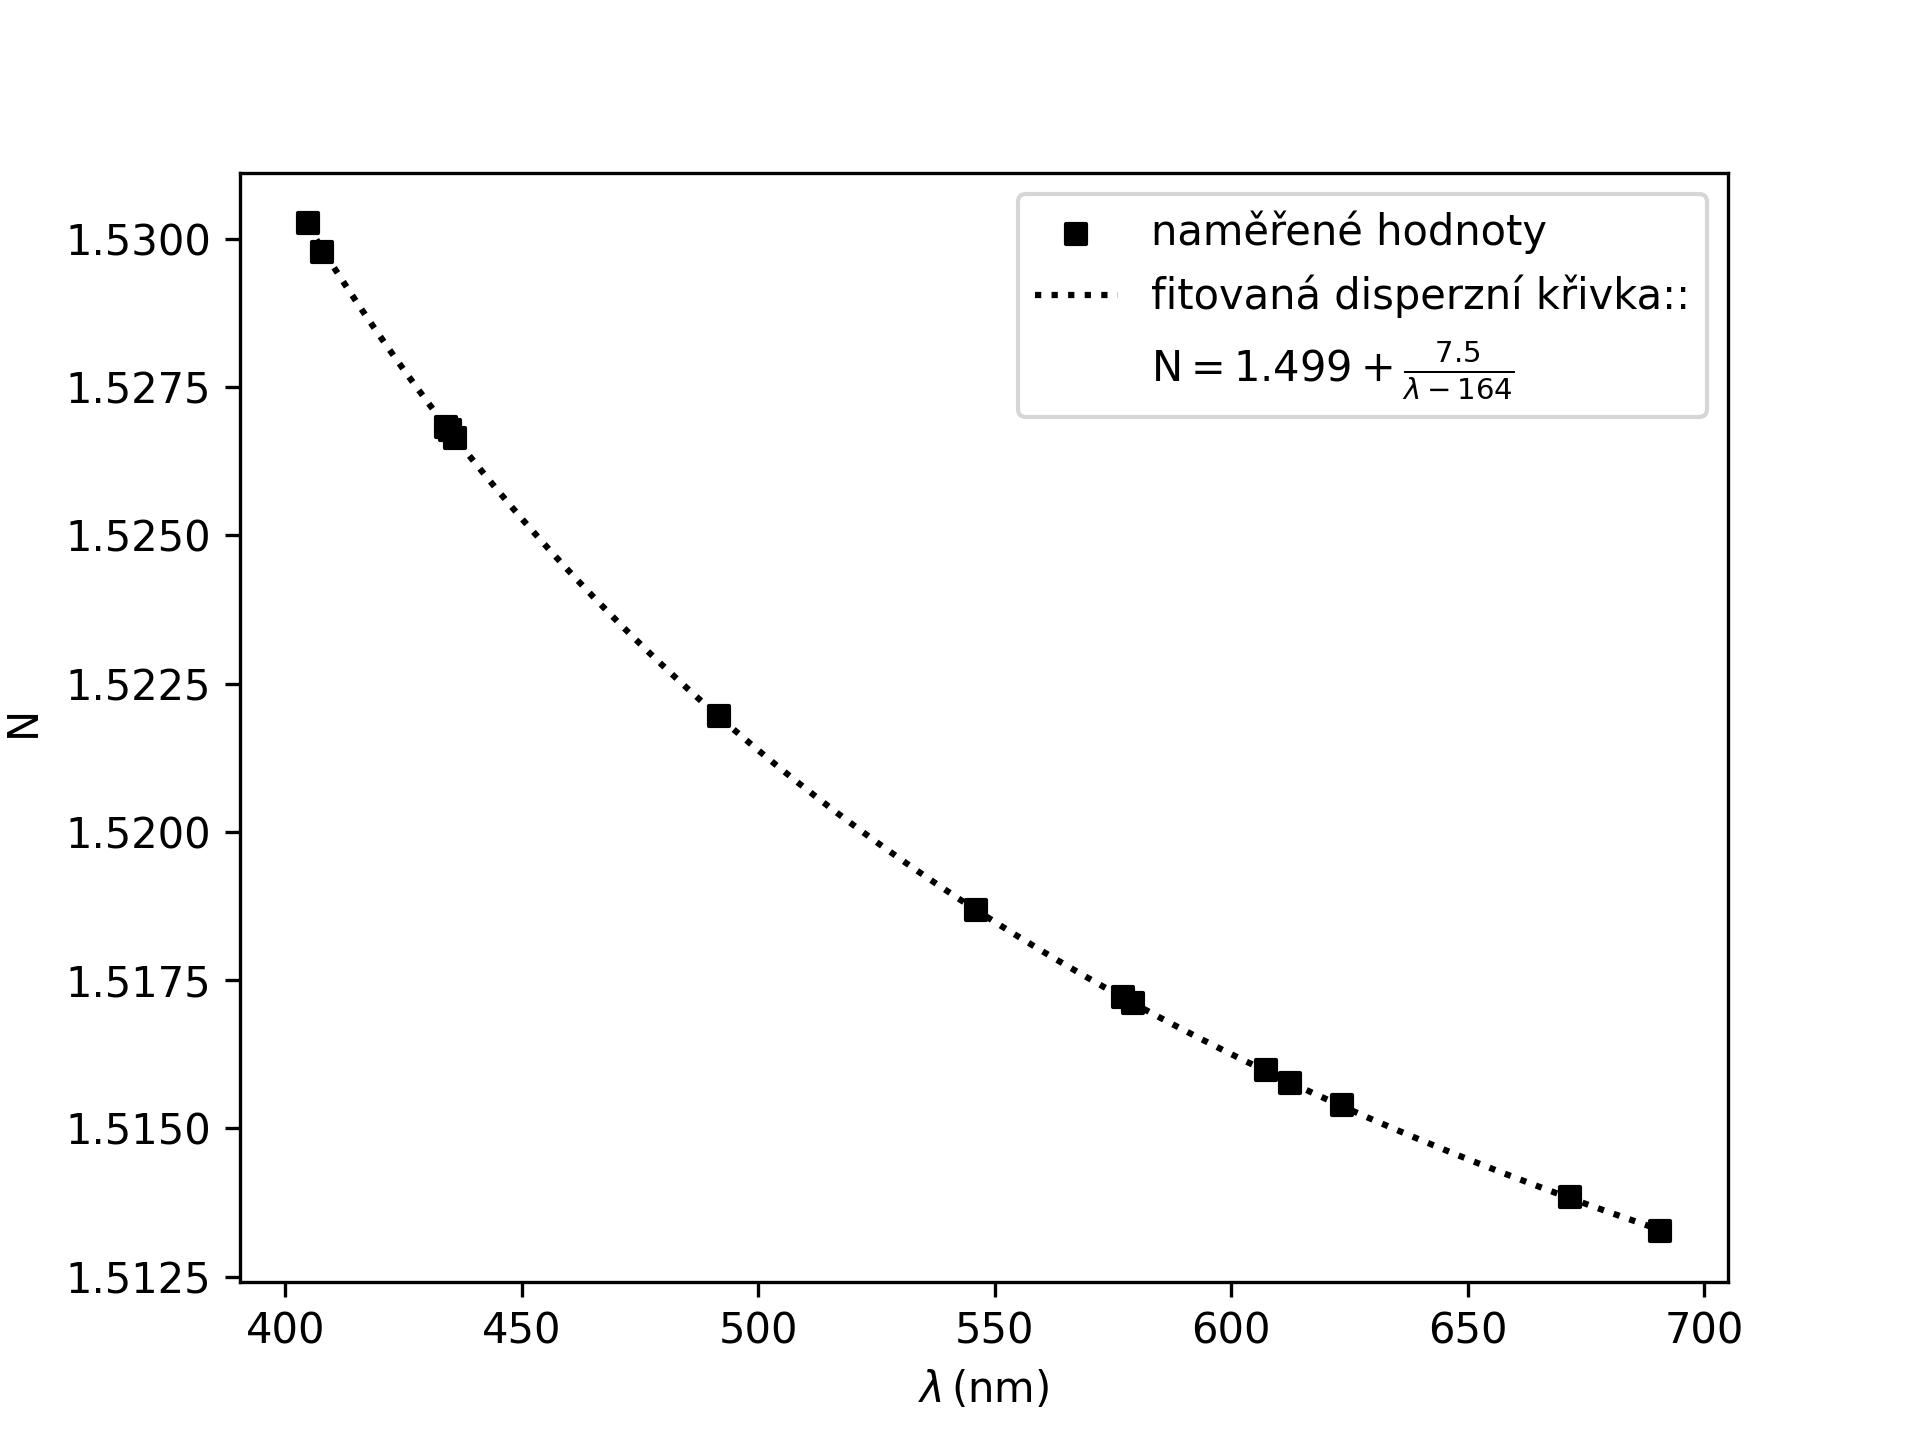
\includegraphics[width=0.7\linewidth]{dispersion.png}
    \caption{Disperzní křivka použitého skleněného hranolu.\nobars}
    \label{fig:dispersion}
\end{figure}

\begin{table}[!htbp]
\centering
\caption{Vlnové délky a indexy lomu významných spektrálních čar}
\begin{tabular}{ccc}
 \toprule
 označení & $\lambda\, (\mathrm{nm})$ & N\\
 \midrule
 C & $656.3$ & $1.5143(5)$ \\
 d & $587.6$ & $1.5168(6)$ \\
 D & $589.3$ & $1.5167(6)$ \\
 F & $486.1$ & $1.5223(8)$ \\
 \bottomrule
\end{tabular}
\label{tab:cdf}
\end{table}

Střední disperze byla z indexů lomu $N_F$ a $N_C$ vypočtena podle vztahu
(\ref{eq:Delta}) a její nejistota jako
\begin{equation}\label{sigmaDelta}
    \sigma_{\Delta} = \sqrt{\sigma_{N_F}^2 + \sigma_{N_C}^2} \, ,
\end{equation}
relativní disperze podle vztahu (\ref{eq:delta}) a její nejistota jako
\begin{equation}\label{sigmadelta}
    \sigma_{\delta} = \sqrt{ \frac{\sigma_{\Delta}^2}
    {\left( N_D - 1 \right)^2} + \frac{\Delta^2 \sigma^2_{N_D}}{\left( N_D - 1 \right)^4} } \, 
\end{equation}
a Abbeovo číslo podle vztahu (\ref{eq:gamma}) a jeho nejistota jako
\begin{equation}\label{sigmagamma}
    \sigma_{\gamma} = \gamma \relative{\delta} \, .
\end{equation}

Hodnoty charakteristických vlastností hranolu jsou uvedeny
v tabulce \ref{tab:vlastnosti}.

\begin{table}[!htbp]
\centering
\caption{Charakteristické vlastnosti skleněného hranolu.}
\begin{tabular}{cc}
 \toprule
 označení & hodnota \\
 \midrule
 $\Delta$ & $0.008(1)$ \\
 $\delta$ & $0.0156(19)$ \\
 $\gamma$ & $64(8)$ \\
 $N_d$ & $1.5168(6)$ \\
 \bottomrule
\end{tabular}
\label{tab:vlastnosti}
\end{table}

% ============================ DISKUZE ===============================
\section{Diskuze}

Podstava použitého hranolu měla tvar rovnostranného trojúhelníku, čemuž
odpovídá naměřený lámavý úhel $\varphi = 60.006(2) \,\degree$ s relativní
nejistotou $3 \cdot 10^{-3}\, \%$. Nejistota je velmi malá, daná jen
nejistotou měření pozic dalekohledu, jež však goniometr umožnil určit
velmi přesně.

Indexy lomu hranolu pro jednotlivé spektrální čáry byly určovány metodou
nalezení minimálního úhlu odklonu. Index lomu je pak dán vztahem (\ref{eq:indexlomu}),
přičemž jeho nejistota závisí na nejistotě lámavého úhlu hranolu 
a~nejistotě minimálního úhlu odklonu podle vzorce (\ref{eq:sigmaN}).
Za předpokladu, že nejistota určení úhlu (mající přímý vliv na nejistotu
lámavého úhlu i úhlu odklonu) je správně odhadnuta, vychází 
pro~všechny měřené čáry nejistota indexu lomu přibližně $5 \cdot 10^{-5}$.
Tato metoda měření tedy zaručuje platnost 4 desetinných míst
hodnoty indexu lomu. Relativní nejistota indexu lomu vychází
přibližně stejně jako relativní nejistota lámavého úhlu.

Některé spektrální čáry byly obtížně viditelné, zejména ty v~červené
oblasti spektra, ale také dvě slabé modré čáry. Při zatemnění místnosti
a díky zkušenosti s vedlejší úlohou (Mřížkový spektrometr) se však
podařilo ve~spektru nalézt všechny čáry specifikované v~tabulce
\cite{tabulka}. Dobře viditelná byla navíc jedna modrozelená čára,
která není v~tabulce uvedena. Tato čára však měla nižší intenzitu.
Opět díky zkušenosti s vedlejší úlohou a také faktu, že disperzní
křivka v grafu \ref{fig:dispersion} prochází přesně všemi naměřenými body
(žádný bod není nad nebo pod křivkou), usuzuji, že byla proměřena
správná modrozelená spektrální čára.

Všechny indexy lomu byly určeny velmi velkou přesností, chybové úsečky
byly dokonce menší než velikost datových bodů. I fitovaná disperzní
křivka (podle vzorce (\ref{eq:disperze})) popisuje naměřená data
velmi dobře. Použití aproximačního vzorce (\ref{eq:disperze}) je
tedy oprávněné.

Z~grafu \ref{fig:dispersion} je patrné, že index lomu
s rostoucí vlnovou délkou klesá, což odpovídá normální disperzi.
Ve~skleněném hranolu tedy nedochází k~absorpci světla. Matematicky
se tato klesající závislost projeví kladným koeficientem $a$ ve~vzorci
(\ref{eq:disperze}). Nejpřesněji byl určen index lomu $N_0 = 1.4990(3)$
s~relativní nejistotou $0.02\,\%$, zbylé dva fitované koeficienty 
$a = 7.5(2)\,\unit{nm^{-1}}$ a $\lambda_0 = -164(5)\,\unit{nm}$ byly
určeny s relativní nejistotou přibližně $3\,\%$. Na~nejistotu 
indexů lomu významných spektrálních čar C, d, D a F měly díky vzorci
(\ref{eq:sigmaN2}) největší vliv nejistoty $N_0$ a $a$. Tyto indexy
lomu se podařilo určit s relativní nejistotou přibližně $0.03\,\%$.

Naopak charakteristické vlastnosti hranolu (parametry $\Delta$, 
$\delta$ a $\gamma$) vycházejí s relativní nejistotou skoro $13\,\%$.
To je dáno tím, že všechny parametry obsahují rozdíl blízkých indexů
lomu $N_F$ a $N_C$. Proto jako hlavní rozlišovací faktor 
mezi různými typy optických skel neuvažuji Abbeovo číslo,
nýbrž~index lomu $N_d$ spektrální čáry d Helia, jež je v tabulce \cite{edmund}
také uveden. Z~tabulky \ref{tab:srovnani} je patrné, že~všechny
vybrané typy optických skel se~svým Abbeovým číslem v~rámci nejistoty
shodují s~použitým hranolem. S přihlédnutím k~indexu lomu $N_d$
se~však jako nejpravděpodobnější typ skla použitého hranolu
jednoznačně jeví \textbf{N-BK7}. Jeho index lomu $N_d$ se~totiž
jako jediný v~rámci nejistoty shoduje s~indexem lomu použitého hranolu.

\begin{table}[!htbp]
\centering
\caption{Srovnání vybraných optických skel z~\cite{edmund} a~použitého
hranolu.}
\begin{tabular}{ccc}
 \toprule
 typ skla & $N_d$ & $\gamma$ \\
 \midrule
 použitý hranol & $1.5168(6)$ & $64(8)$ \\
 S-FSL5 & $1.487$ & $70.20$ \\
 N-BK7 & $1.517$ & $64.20$ \\
 N-K5 & $1.522$ & $59.50$ \\
 B270/S1 & $1.523$ & $58.50$ \\
 N-SK11 & $1.564$ & $60.80$ \\
 \bottomrule
\end{tabular}
\label{tab:srovnani}
\end{table}

% ============================= ZÁVĚR ================================
\section{Závěr}

Lámavý úhel hranolu byl určen jako $\varphi = 60.006(2) \,\degree$.

Metoda měření indexu lomu pomocí minimálního úhlu odklonu umožňuje
určit index lomu s~přesností na~4 desetinná místa.

Použitý skleněný hranol vykazuje normální disperzi, naměřenou
závislost indexu lomu na~vlnové délce lze s~dobrou přesností
popsat funkcí ve~tvaru (\ref{eq:disperze}), přičemž koeficient $a$ je kladný.

Nakonec byly určeny disperzní vlastnosti použitého hranolu:
\begin{itemize}
    \item střední disperze: $\Delta = 0.008(1)$
    \item relativní disperze: $\delta = 0.0156(19)$
    \item Abbeovo číslo: $\gamma = 64(8)$
    \item index lomu d čáry Helia: $N_d = 1.5168(6)$\,.
\end{itemize}
Těmto hodnotám odpovídá optické sklo typu N-BK7.

% =========================== LITERATURA =============================
\renewcommand{\today}{\number\day.\,\number\month.\,\number\year}
\begin{thebibliography}{9}

\bibitem{pokyny} Kolektiv ZFP KVOF MFF UK: \textit{Měření indexu lomu Fraunhoferovou
metodou - pokyny k měření} [online]. [cit. \today], dostupné 
z~https://physics.mff.cuni.cz/vyuka/zfp/\_media/zadani/pokyny/mereni\_316.pdf

\bibitem{studijni} Kolektiv ZFP KVOF MFF UK: \textit{Měření indexu lomu Fraunhoferovou 
metodou - studijní text} [online]. \\ 
\text{[cit. \today]}, 
dostupné z~https://physics.mff.cuni.cz/vyuka/zfp/\_media/zadani/texty/txt\_316.pdf

\bibitem{englich} J. Englich: \textit{Úvod do praktické fyziky I: Zpracování výsledků měření}. 
1. vyd. Praha: Matfyzpress, 2006

\bibitem{tabulka} Kolektiv ZFP KVOF MFF UK: \textit{Tabulka spektrálních čar rtuti} [online]. 
[cit. \today],
dostupné 
z~https://physics.mff.cuni.cz/vyuka/zfp/\_media/zadani/pokyny/tabulka\_spektralnich\_car\_rtuti.pdf

\bibitem{edmund} Edmund Optics Inc.: \textit{Optical Glass - Optical Glass Properties}
[online]. \text{[cit. \today]}, \\
dostupné z~https://www.edmundoptics.com/knowledge-center/application-notes/optics/optical-glass/?srsltid=AfmBOopxB6NqJZ8\_RdpDI8HsBD3Py-egl1W7G153jfHfNS9F-XUjXg9L

\end{thebibliography}
\end{document}